\documentclass[a4paper]{article}
\usepackage{graphicx} 
\usepackage{float} 
\usepackage{subfigure}
\usepackage{amsmath}
\usepackage{indentfirst}
\title{Scientific Computing HW2}
\author{Runze Fang}
\date{\today}

\begin{document}
\maketitle
\section{The Hilber Matrix}
\subsection{Conditioning Numbers}
Fristly I compared direct calculation of condition number with the built-in exact calculation cond.

\begin{figure}[H] 
\centering 
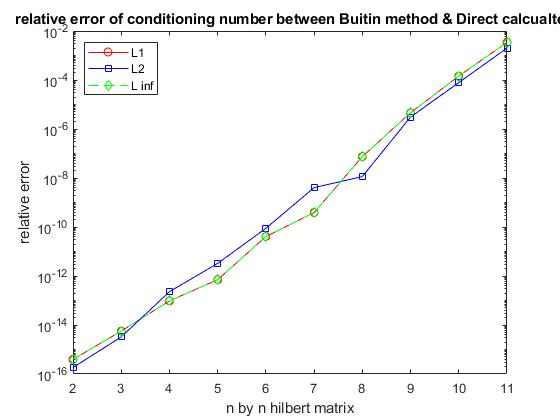
\includegraphics[width=1.0\textwidth]{1.1-1.png}
\caption{condition number comparation} 
\label{Fig.1.1-1} 
\end{figure}

As shown in  Figure 1, the relative error of computing condition number directly increase with the size of hilbert
matrix increasing. Each time the hilbert matrix size increases, we lose 2 digits of accuracy. The graph also shows
that the built in function has the same result with direct calculating when calculating L1 and L infinite
, while it does not when calculating L2. This observation in accordance with Matlab document: when doing L2, cond
method use Singular Value Decomposition to do the calculation.

\indent Then I compared direct calculation of reciprocal condition number with the estimate rond number.

\begin{figure}[H] 
\centering 
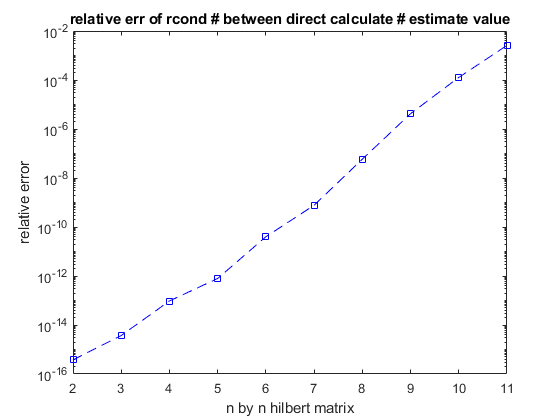
\includegraphics[width=1.0\textwidth]{1.1-2.png}
\caption{reciprocal condition number comparation} 
\label{Fig.1.1-2} 
\end{figure}

As shown in Figure 2, the relative error of computing reciprocal condition number increase with the size of hilbert
matrix increasing. Each time the hilbert matrix size increases, we also lose 2 digits of accuracy.

\subsection{Solving ill-conditioned systems}
I first solve the linear system by using the built-in solver: $linsolve$. According to the document, it use LU factorization 
to solve the system. Then I calculate the relative error using the infinite norm. I did the same procedure using Cholesky 
factorization. Also, I compute the residual under these two senario.

\begin{figure}[H] 
\centering 
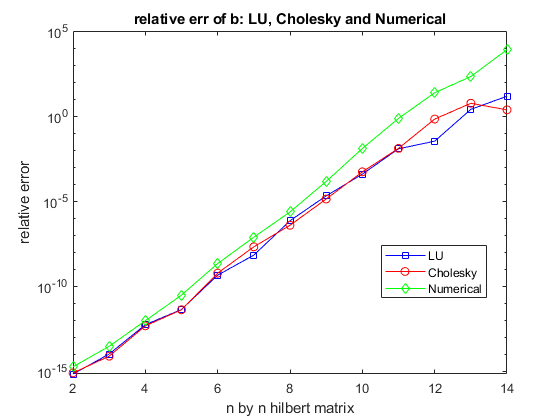
\includegraphics[width=1.0\textwidth]{1.2-1.png}
\caption{relative error of b by using factorization and numerical computing} 
\label{Fig.1.2-1} 
\end{figure}

\begin{figure}[H] 
\centering 
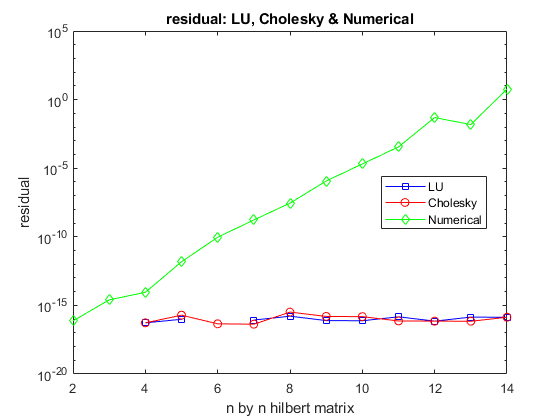
\includegraphics[width=1.0\textwidth]{1.2-2.png}
\caption{residual by using factorization and numerical computing} 
\label{Fig.1.2-2} 
\end{figure}
As shown in Figure 3, the number of digit accuracy decreases as the size of hilbert matrix increasing. Every time the size of Hilbert
matrix increase by 1, we lose 1 to 2 digits of accuracy. When $n > 12$ we canot get any digit of accuracy. The relative error diverges after $6\times 6$ hilbert matrix. This observation comforms with what we can see in Figure 4: the residual calculated by LU factorization of $6\times 6$ hilbert matrix equals 0, which is abnormal. The trend of residual value conformed with the trend of condition number: when $n \leq 3$, the condition number is relatively large, the matrix is reletive stable, therefore, the residuals are 0; when $n \geq 4$, there are residuals. As for conclusion, LU factorization and Cholesky factorization has nearly the same performance: they share
 the same large of residual, and close relative error. However, after 6 by 6 hilbert matrix, Choleskey factorization seems slightly more stable.\\
\indent The result confoms to the theoretical expectation discussed in class. After $n=12$, it no longer make sense to even try solving the system due to the sever ill-condition\\
\indent Then I compute the solution by using the numerically-computed matrix inverse function $matinv$. Also shown in Figure 3 and 4,
I compared numerical method, LU and Cholesky factorization together. Considering the relative error, the numerical method lose at least one more digit of accuracy than both factorizations. As the size of hilbert matrix grows, the numerical method will lose more digits of accuracy. Considering the residual, numerical method has way larger residual then the factorizations have. Therefore, LU and Cholesky factorizations are way better than the numerical method.\\
\indent Finally, I compared the $matinv$ function and $invhilb$ function.

\begin{figure}[H] 
\centering 
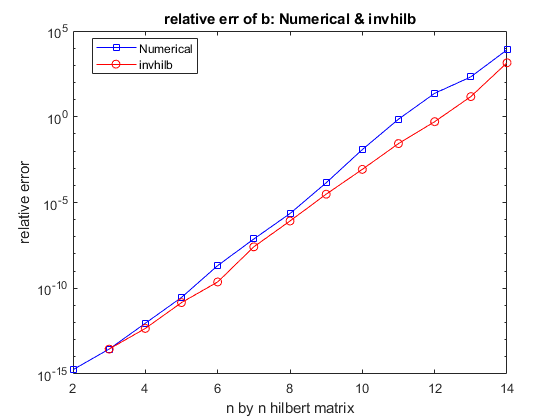
\includegraphics[width=1.0\textwidth]{1.2-3.png}
\caption{relative error of different numerical method} 
\label{Fig.1.2-3} 
\end{figure}

\begin{figure}[H] 
\centering 
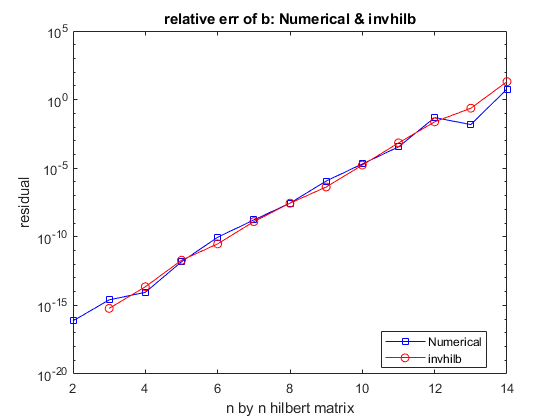
\includegraphics[width=1.0\textwidth]{1.2-4.png}
\caption{residual by using different numerical method} 
\label{Fig.1.2-4} 
\end{figure}
As shown in Figure 5 and Figure 6, $matinv$ and $invhilb$ has the same large residuals. Comparing the relative errors, when the size of the matrix is larger than 6, the $invhilb$ gets at least 1 digits of accuracy. Therefore, using $invhilb$ is more optimal when doing numerical computing. This might be because 3 sets of roundoff errors. Firstly, when doing $inv(hilb(n))$, there will be error representing $hilb(n)$. Secondly, when doing inversion, there will be errors. Finally, there is error when representing $invhilb(n)$. The $invhilb$ method may have less error in the first senario.

\section{Different Methods}
\subsection{Three-method fitting}
I estimate $\tilde{c}$ and generate $\lVert c - \tilde{c}\rVert$ for different $\epsilon$ in three ways: using the built-in function $polyfit$, using backslash operator and forming the system of normal equations. 
\begin{figure}[H] 
\centering 
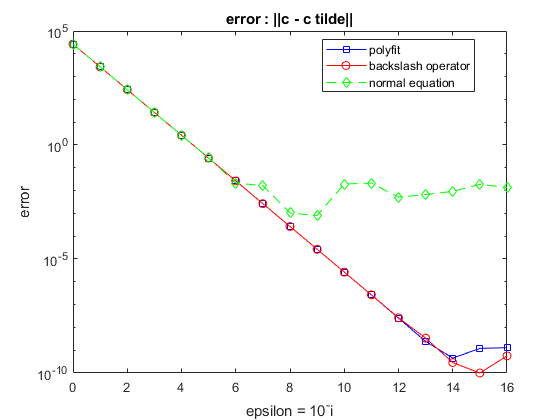
\includegraphics[width=1.0\textwidth]{2.1-1.png}
\caption{error: norm of ( c - c tilda )} 
\label{Fig.2.1-1} 
\end{figure}

\begin{figure}[H] 
\centering 
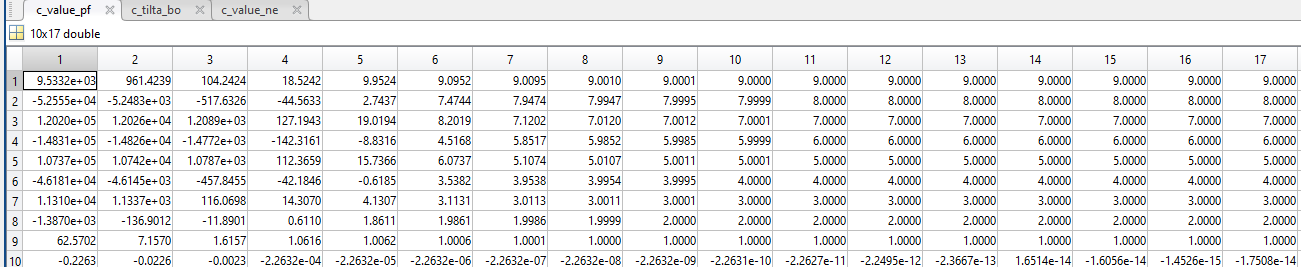
\includegraphics[width=1.0\textwidth]{2.1-2.png}
\caption{estimate coefficient by polyfit} 
\label{Fig.2.1-2} 
\end{figure}

\begin{figure}[H] 
\centering 
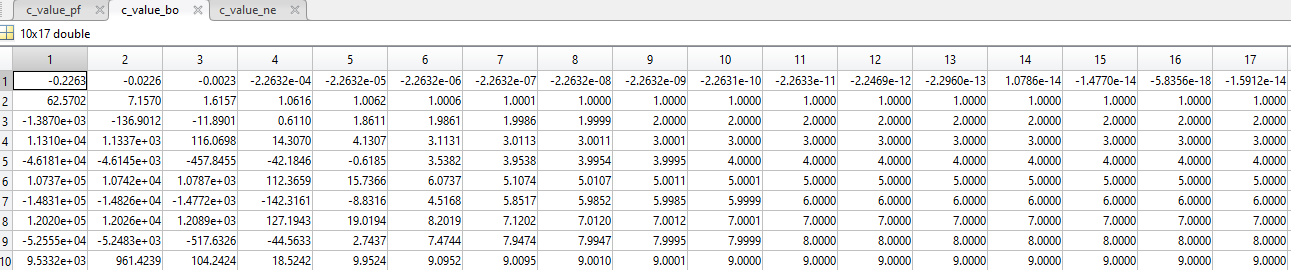
\includegraphics[width=1.0\textwidth]{2.1-3.png}
\caption{estimate coefficient by backslash} 
\label{Fig.2.1-3} 
\end{figure}

\begin{figure}[H] 
\centering 
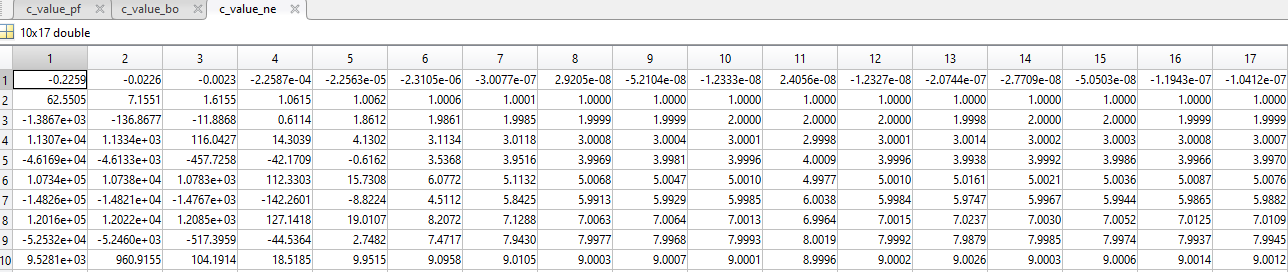
\includegraphics[width=1.0\textwidth]{2.1-4.png}
\caption{estimate coefficient by norm equations} 
\label{Fig.2.1-4} 
\end{figure}

As shown in Figure 7, the error computed by $polyfit$ and backslash operator performs the same error. These two senario diverges from $\epsilon = 10^{-14}$. This may because when $\epsilon$ is close to the maximum accuracy of double, the roundoff error occurs.
The error of normal equation diverges from the above two methods when $i \geq 6$. This may because of when doing $A^{T}A$ and $A^{T}y$,  we have a huge round off error. In contrast, we did not perform any multiplication using the backslash operator to solve the linear system. Therefore, the normal equation method has a big error when $i \geq 6$.


\subsection{The Best Method}
If $\epsilon = 0$, we get the exact result of fitting. I compute the exact result of fitting using 3 method and the result is shown below.

\begin{figure}[H] 
\centering 
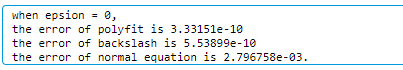
\includegraphics[width=1.0\textwidth]{2.1-5.png}
\caption{exact result of fitting} 
\label{Fig.2.1-5} 
\end{figure}

As shown in Figure 11, the highest accuracy I can achieve is 10 digits of accuracy. The $polyfit$ method and the backslash method share the same performance, while the normal equation is obvious inferior to the previos two methods. This result conforms with my discussion in 2.1: the normal equation method has huge roundoff error due to the multiplication of $A^{T}A$ and $A^{T}y$.\\
\indent Empirically, as the degree $d$ increases, the system becomes more ill-conditioned. The more degrees means the $A^{T}A$ matrix becomes ill-conditioned and as our computation becomes more complex, more roundoff error are introduced. As a result, $(A^{T}A)^{-1}$ will be estimated with a huge error. Thus, the overdetermined linear system becomes more ill-conditioned.

\section{Rank-1 Matrix Updates}
\subsection{Direct Update}
I generate a $5 \times 5$ matrix $A$ and a $rhs$ by using $randn$, and then I solve $Ax=b$. Then I generate two vetors $u$ and $v$ to updated the system, then compute the residual $r=b-\tilde{A}\tilde{x}$. The generated matrices and the residual are shown below.

\begin{figure}[H] 
\centering 
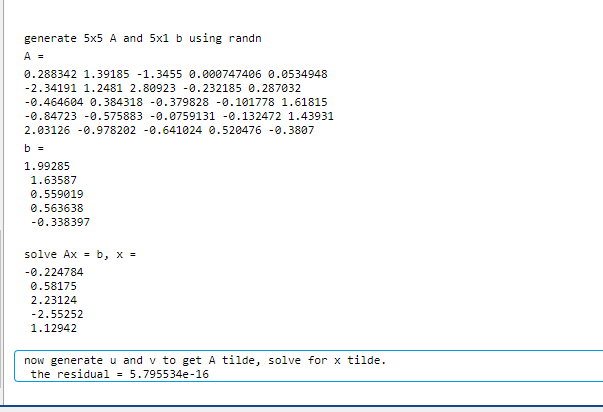
\includegraphics[width=1.0\textwidth]{3.1-1.png}
\caption{generated matrices, x and residual r} 
\label{Fig.3.1-1} 
\end{figure}

As shown in Figure 12, the residual is around $5e-16$, which is close to the lower bundary of double and it is very small.
\subsection{SMW Formula}
I generated a $100\times100$ matrix $A$ and compute $\tilde{x}$ in two ways: direct computing and using SMW formula. Then I compute the norm of these two $\tilde{x}$. The result is shown below.

\begin{figure}[H] 
\centering 
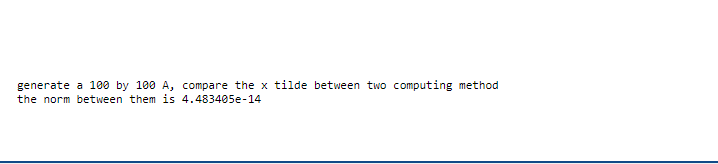
\includegraphics[width=1.0\textwidth]{3.2-1.png}
\caption{norm of x tilde computed in different ways} 
\label{Fig.3.2-1} 
\end{figure}

The norm between two $\tilde{x}$ computed in two diferent ways is about $4e-14$, which indicates the gap between them is not big.\\
\indent If we use the SMW formula to compute $\tilde{x}=\tilde{A}^{-1}b$, we can solve it more efficiently giving the condition that we has already know the LU factorization of $A$. This will requires $O(n^{2})$ work. Using the SMW formula we get\\
$\tilde{x}=\tilde{A}^{-1}b=A^{-1}b-\frac{A^{-1}uv^{T}A^{-1}b}{1+v^{T}A^{-1}u}$.\\
Let $Az = u$ for $z$, so $z=A^{-1}u$. This will have $FLOPS\approx{2n^2}$, since the forward substitution and the backward substitution will have a $FLOPS\approx{n^2}$ for each. And let $Ay = b$ for $y$, so $y=A^{-1}b$. This will also have $FLOPS\approx{2n^2}$. These two procedure will have a total $FLOPS\approx{4n^2}$.\\
\indent Now we can compute $\tilde{x}= y-\frac{zv^{T}y}{1+v^{T}z}$. The procedure $zv^{T}$ will have $FLOPS\approx{n^2}$ because it is a $n\times{1}$ matrix multiply a $1\times{n}$ matrix and get an $n\times{n}$ matrix.
Then, the procedure $zv^{T}y$ will have a $FLOPS \approx{n(2n-1)}$. Similarly, to perform $v^{T}z$, we will have $FLOPS \approx{2n-1}$. Adding all flops together with one adding operation, one subtractiong operaton and one dividing operation, we get a total $FLOPS \approx{7n^{2} +2n}$.\\
\indent In comparison, solving $\tilde{A}\tilde{x}=b$ directly will have a $FLOP \approx{\frac{2}{3}n^{3}+4n^{2}}$, since it has one LU fratorization and two backslash operations.\\
\indent In conclusion, computing directly is $O(n^3)$, while the implementation of SMW formula is $O(n^2)$, the later is way faster than the former. This is because if A is already factored, we only do triangular solutions and inner products, while when we compute directly, we will do one more step of explicity inverses.
\end{document}